\documentclass{standalone}
\usepackage{tikz}
\usetikzlibrary{patterns, positioning}


\begin{document}
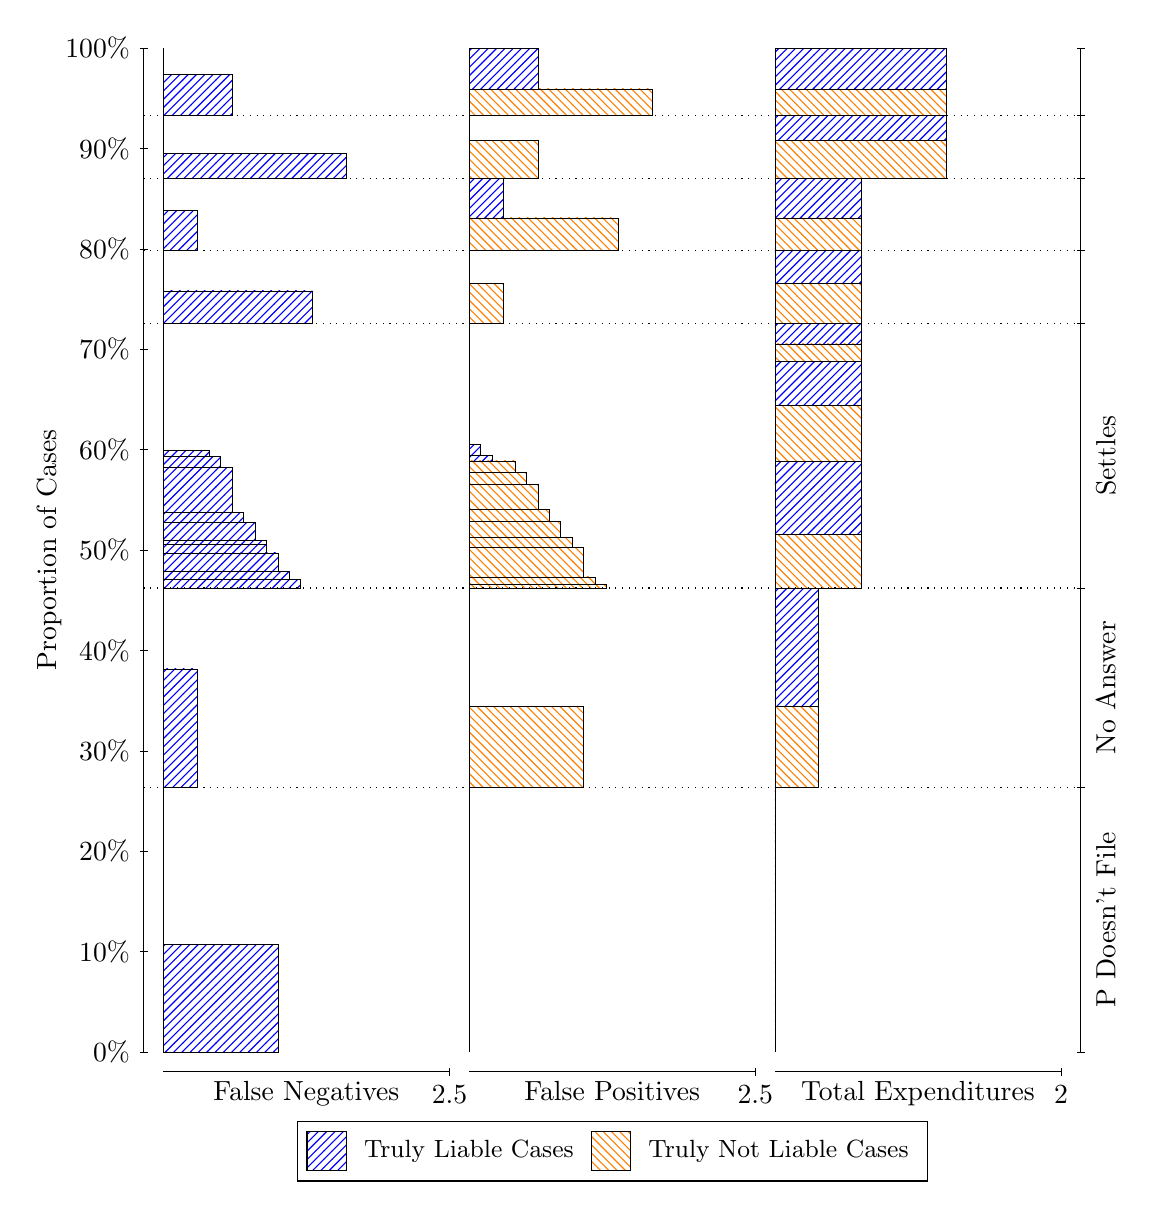
\begin{tikzpicture}
\draw[black, very thin] (1.5,1.75) -- (1.5,14.5);
\node[rotate=90, text=black, anchor=center] at (0.3, 8.125) {Proportion of Cases};
\draw[black, very thin] (1.45,1.75) -- (1.55,1.75);
\node[text=black, anchor=east] at (1.45, 1.75) {0\%};
\draw[black, very thin] (1.45,3.025) -- (1.55,3.025);
\node[text=black, anchor=east] at (1.45, 3.025) {10\%};
\draw[black, very thin] (1.45,4.3) -- (1.55,4.3);
\node[text=black, anchor=east] at (1.45, 4.3) {20\%};
\draw[black, very thin] (1.45,5.575) -- (1.55,5.575);
\node[text=black, anchor=east] at (1.45, 5.575) {30\%};
\draw[black, very thin] (1.45,6.85) -- (1.55,6.85);
\node[text=black, anchor=east] at (1.45, 6.85) {40\%};
\draw[black, very thin] (1.45,8.125) -- (1.55,8.125);
\node[text=black, anchor=east] at (1.45, 8.125) {50\%};
\draw[black, very thin] (1.45,9.4) -- (1.55,9.4);
\node[text=black, anchor=east] at (1.45, 9.4) {60\%};
\draw[black, very thin] (1.45,10.675) -- (1.55,10.675);
\node[text=black, anchor=east] at (1.45, 10.675) {70\%};
\draw[black, very thin] (1.45,11.95) -- (1.55,11.95);
\node[text=black, anchor=east] at (1.45, 11.95) {80\%};
\draw[black, very thin] (1.45,13.225) -- (1.55,13.225);
\node[text=black, anchor=east] at (1.45, 13.225) {90\%};
\draw[black, very thin] (1.45,14.5) -- (1.55,14.5);
\node[text=black, anchor=east] at (1.45, 14.5) {100\%};

\draw[black, very thin] (13.4,1.75) -- (13.4,14.5);
\draw[black, very thin] (13.35,1.75) -- (13.45,1.75);
\node[anchor=west] at (13.35, 1.75) {};
\draw[black, very thin] (13.35,5.1112) -- (13.45,5.1112);
\node[anchor=west] at (13.35, 5.1112) {};
\draw[black, very thin] (13.35,7.6419) -- (13.45,7.6419);
\node[anchor=west] at (13.35, 7.6419) {};
\draw[black, very thin] (13.35,11.001) -- (13.45,11.001);
\node[anchor=west] at (13.35, 11.001) {};
\draw[black, very thin] (13.35,11.93) -- (13.45,11.93);
\node[anchor=west] at (13.35, 11.93) {};
\draw[black, very thin] (13.35,12.848) -- (13.45,12.848);
\node[anchor=west] at (13.35, 12.848) {};
\draw[black, very thin] (13.35,13.645) -- (13.45,13.645);
\node[anchor=west] at (13.35, 13.645) {};
\draw[black, very thin] (13.35,14.5) -- (13.45,14.5);
\node[anchor=west] at (13.35, 14.5) {};

\draw[black, very thin, pattern color=blue, pattern=north east lines] (1.75,1.75) rectangle (3.2033,3.1181);
\draw[black, very thin, pattern color=orange, pattern=north west lines] (1.75,3.1181) rectangle (1.75,5.1112);
\draw[black, very thin, pattern color=blue, pattern=north east lines] (1.75,5.1112) rectangle (2.186,6.6163);
\draw[black, very thin, pattern color=orange, pattern=north west lines] (1.75,6.6163) rectangle (1.75,7.6419);
\draw[black, very thin, pattern color=blue, pattern=north east lines] (1.75,7.6419) rectangle (3.494,7.7478);
\draw[black, very thin, pattern color=blue, pattern=north east lines] (1.75,7.7478) rectangle (3.3487,7.8546);
\draw[black, very thin, pattern color=blue, pattern=north east lines] (1.75,7.8546) rectangle (3.2033,8.087);
\draw[black, very thin, pattern color=blue, pattern=north east lines] (1.75,8.087) rectangle (3.058,8.1949);
\draw[black, very thin, pattern color=blue, pattern=north east lines] (1.75,8.1949) rectangle (3.058,8.2469);
\draw[black, very thin, pattern color=blue, pattern=north east lines] (1.75,8.2469) rectangle (2.9127,8.4708);
\draw[black, very thin, pattern color=blue, pattern=north east lines] (1.75,8.4708) rectangle (2.7673,8.6039);
\draw[black, very thin, pattern color=blue, pattern=north east lines] (1.75,8.6039) rectangle (2.622,9.1718);
\draw[black, very thin, pattern color=blue, pattern=north east lines] (1.75,9.1718) rectangle (2.4767,9.3115);
\draw[black, very thin, pattern color=blue, pattern=north east lines] (1.75,9.3115) rectangle (2.3313,9.3856);
\draw[black, very thin, pattern color=orange, pattern=north west lines] (1.75,9.3856) rectangle (1.75,11.001);
\draw[black, very thin, pattern color=blue, pattern=north east lines] (1.75,11.001) rectangle (3.6393,11.417);
\draw[black, very thin, pattern color=orange, pattern=north west lines] (1.75,11.417) rectangle (1.75,11.93);
\draw[black, very thin, pattern color=blue, pattern=north east lines] (1.75,11.93) rectangle (2.186,12.434);
\draw[black, very thin, pattern color=orange, pattern=north west lines] (1.75,12.434) rectangle (1.75,12.848);
\draw[black, very thin, pattern color=blue, pattern=north east lines] (1.75,12.848) rectangle (4.0753,13.165);
\draw[black, very thin, pattern color=orange, pattern=north west lines] (1.75,13.165) rectangle (1.75,13.645);
\draw[black, very thin, pattern color=blue, pattern=north east lines] (1.75,13.645) rectangle (2.622,14.165);
\draw[black, very thin, pattern color=orange, pattern=north west lines] (1.75,14.165) rectangle (1.75,14.5);
\draw[black, very thin, pattern color=orange, pattern=north west lines] (5.6333,1.75) rectangle (5.6333,3.7431);
\draw[black, very thin, pattern color=blue, pattern=north east lines] (5.6333,3.7431) rectangle (5.6333,5.1112);
\draw[black, very thin, pattern color=orange, pattern=north west lines] (5.6333,5.1112) rectangle (7.0867,6.1368);
\draw[black, very thin, pattern color=blue, pattern=north east lines] (5.6333,6.1368) rectangle (5.6333,7.6419);
\draw[black, very thin, pattern color=orange, pattern=north west lines] (5.6333,7.6419) rectangle (7.3773,7.6908);
\draw[black, very thin, pattern color=orange, pattern=north west lines] (5.6333,7.6908) rectangle (7.232,7.7844);
\draw[black, very thin, pattern color=orange, pattern=north west lines] (5.6333,7.7844) rectangle (7.0867,8.1598);
\draw[black, very thin, pattern color=orange, pattern=north west lines] (5.6333,8.1598) rectangle (6.9413,8.2816);
\draw[black, very thin, pattern color=orange, pattern=north west lines] (5.6333,8.2816) rectangle (6.796,8.4922);
\draw[black, very thin, pattern color=orange, pattern=north west lines] (5.6333,8.4922) rectangle (6.6507,8.6399);
\draw[black, very thin, pattern color=orange, pattern=north west lines] (5.6333,8.6399) rectangle (6.5053,8.962);
\draw[black, very thin, pattern color=orange, pattern=north west lines] (5.6333,8.962) rectangle (6.36,9.1063);
\draw[black, very thin, pattern color=orange, pattern=north west lines] (5.6333,9.1063) rectangle (6.2147,9.2569);
\draw[black, very thin, pattern color=blue, pattern=north east lines] (5.6333,9.2569) rectangle (5.924,9.331);
\draw[black, very thin, pattern color=blue, pattern=north east lines] (5.6333,9.331) rectangle (5.7787,9.4707);
\draw[black, very thin, pattern color=blue, pattern=north east lines] (5.6333,9.4707) rectangle (5.6333,11.001);
\draw[black, very thin, pattern color=orange, pattern=north west lines] (5.6333,11.001) rectangle (6.0693,11.513);
\draw[black, very thin, pattern color=blue, pattern=north east lines] (5.6333,11.513) rectangle (5.6333,11.93);
\draw[black, very thin, pattern color=orange, pattern=north west lines] (5.6333,11.93) rectangle (7.5227,12.343);
\draw[black, very thin, pattern color=blue, pattern=north east lines] (5.6333,12.343) rectangle (6.0693,12.848);
\draw[black, very thin, pattern color=orange, pattern=north west lines] (5.6333,12.848) rectangle (6.5053,13.328);
\draw[black, very thin, pattern color=blue, pattern=north east lines] (5.6333,13.328) rectangle (5.6333,13.645);
\draw[black, very thin, pattern color=orange, pattern=north west lines] (5.6333,13.645) rectangle (7.9587,13.98);
\draw[black, very thin, pattern color=blue, pattern=north east lines] (5.6333,13.98) rectangle (6.5053,14.5);
\draw[black, very thin, pattern color=orange, pattern=north west lines] (9.5167,1.75) rectangle (9.5167,3.7431);
\draw[black, very thin, pattern color=blue, pattern=north east lines] (9.5167,3.7431) rectangle (9.5167,5.1112);
\draw[black, very thin, pattern color=orange, pattern=north west lines] (9.5167,5.1112) rectangle (10.062,6.1368);
\draw[black, very thin, pattern color=blue, pattern=north east lines] (9.5167,6.1368) rectangle (10.062,7.6419);
\draw[black, very thin, pattern color=orange, pattern=north west lines] (9.5167,7.6419) rectangle (10.607,8.3215);
\draw[black, very thin, pattern color=blue, pattern=north east lines] (9.5167,8.3215) rectangle (10.607,9.2531);
\draw[black, very thin, pattern color=orange, pattern=north west lines] (9.5167,9.2531) rectangle (10.607,9.9643);
\draw[black, very thin, pattern color=blue, pattern=north east lines] (9.5167,9.9643) rectangle (10.607,10.517);
\draw[black, very thin, pattern color=orange, pattern=north west lines] (9.5167,10.517) rectangle (10.607,10.742);
\draw[black, very thin, pattern color=blue, pattern=north east lines] (9.5167,10.742) rectangle (10.607,11.001);
\draw[black, very thin, pattern color=orange, pattern=north west lines] (9.5167,11.001) rectangle (10.607,11.513);
\draw[black, very thin, pattern color=blue, pattern=north east lines] (9.5167,11.513) rectangle (10.607,11.93);
\draw[black, very thin, pattern color=orange, pattern=north west lines] (9.5167,11.93) rectangle (10.607,12.343);
\draw[black, very thin, pattern color=blue, pattern=north east lines] (9.5167,12.343) rectangle (10.607,12.848);
\draw[black, very thin, pattern color=orange, pattern=north west lines] (9.5167,12.848) rectangle (11.697,13.328);
\draw[black, very thin, pattern color=blue, pattern=north east lines] (9.5167,13.328) rectangle (11.697,13.645);
\draw[black, very thin, pattern color=orange, pattern=north west lines] (9.5167,13.645) rectangle (11.697,13.98);
\draw[black, very thin, pattern color=blue, pattern=north east lines] (9.5167,13.98) rectangle (11.697,14.5);
\draw[black, dotted] (1.5,5.1112) -- (13.4,5.1112);
\draw[black, dotted] (1.5,7.6419) -- (13.4,7.6419);
\draw[black, dotted] (1.5,11.001) -- (13.4,11.001);
\draw[black, dotted] (1.5,11.93) -- (13.4,11.93);
\draw[black, dotted] (1.5,12.848) -- (13.4,12.848);
\draw[black, dotted] (1.5,13.645) -- (13.4,13.645);
\draw[black, very thin] (1.75,1.5) -- (5.3833,1.5);
\node[text=black, anchor=north] at (3.5667, 1.5) {False Negatives};
\draw[black, very thin] (5.3833,1.45) -- (5.3833,1.55);
\node[text=black, anchor=north] at (5.3833, 1.45) {2.5};

\draw[black, very thin] (5.6333,1.5) -- (9.2667,1.5);
\node[text=black, anchor=north] at (7.45, 1.5) {False Positives};
\draw[black, very thin] (9.2667,1.45) -- (9.2667,1.55);
\node[text=black, anchor=north] at (9.2667, 1.45) {2.5};

\draw[black, very thin] (9.5167,1.5) -- (13.15,1.5);
\node[text=black, anchor=north] at (11.333, 1.5) {Total Expenditures};
\draw[black, very thin] (13.15,1.45) -- (13.15,1.55);
\node[text=black, anchor=north] at (13.15, 1.45) {2};

\node[text=black, centered, rotate=90] at (13.72, 3.4306) {P Doesn't File};
\node[text=black, centered, rotate=90] at (13.72, 6.3765) {No Answer};
\node[text=black, centered, rotate=90] at (13.72, 9.3213) {Settles};





\draw (7.449999999999999,1.5) node[draw=none] (baseCoordinate) {};
\begin{scope}[align=center]
        \matrix[scale=0.5, draw=black, below=0.5cm of baseCoordinate, nodes={draw}, column sep=0.1cm]{
            \node[rectangle, draw, minimum width=0.5cm, minimum height=0.5cm, pattern color=blue, pattern=north east lines] {}; &
            \node[draw=none, font=\small, text=black] (B) {Truly Liable Cases}; &
            \node[rectangle, draw, minimum width=0.5cm, minimum height=0.5cm, pattern color=orange, pattern=north west lines] {}; &
            \node[draw=none, font=\small, text=black] (B) {Truly Not Liable Cases}; \\
            };
\end{scope}

\end{tikzpicture}
\end{document}